TJ-Monopix1 is a small electrode DMAPS with fast R/O capability, fabricated by TowerJazz foundry in 180 nm CMOS imaging process.
It is part, together with prototypes from other series such as TJ-MALTA, of the ongoing R$\&$D efforts aimed at developing DMAPS in commercial CMOS processes, that could cope with the requirements at accelerator experiments.
Both TJ-Monopix and TJ-MALTA series \cite{MALTA}, produced with the same technology by TowerJazz (the timeline of the foundry products is shown in figure \ref{fig:TJ180nm}), are small electrode demonstrators and principally differ in the readout design: while Monopix implements a column-drain R/O, an asynchronous R/O without any distribution of BCID has been used by TJ-Malta in order to reduce power consumption.

\begin{figure}[h!]
    \centering
    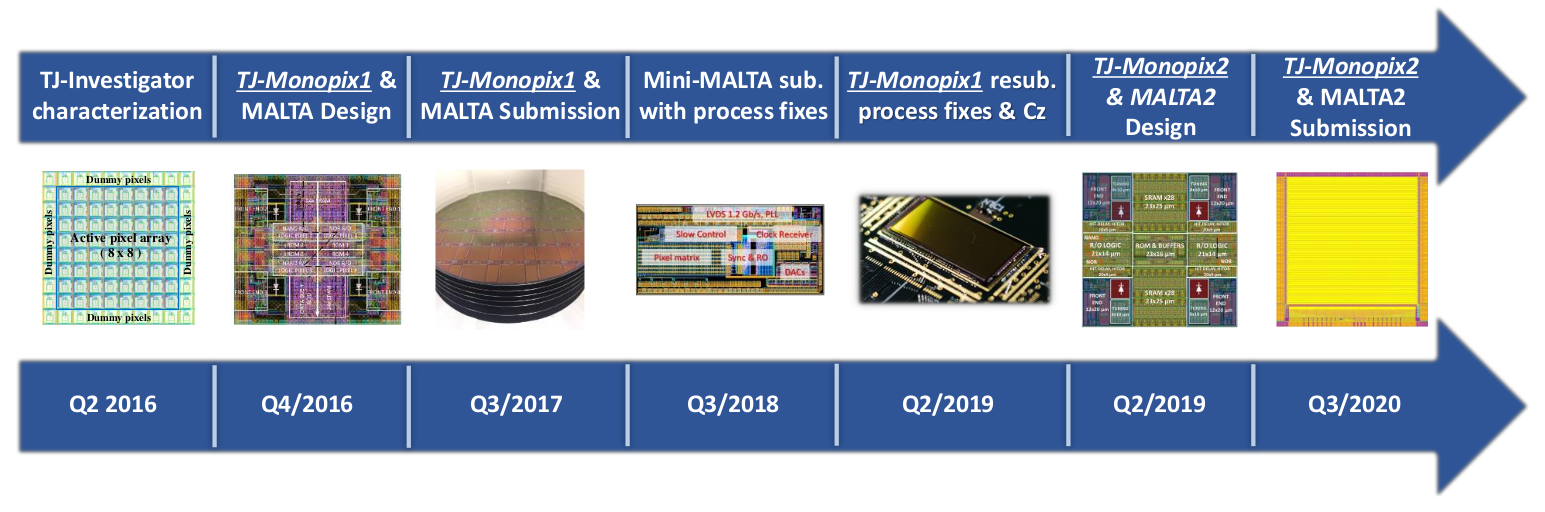
\includegraphics[width=.95\linewidth]{figures/Monopix1/TJ180nm.png}
    \caption{Timeline in TowerJazz productions in 180 nm CMOS imaging process}
    \label{fig:TJ180nm}
\end{figure} 

Another Monopix series, but in 150 nm CMOS technology, has been produced by LFoundry~\cite{LF-Monopix}.
The main differences between the LF-Monopix1 and the TJ-Monopix1 (summarized in table \ref{tab:LF-TJ-Monopix}), lay in the sensor rather than in the readout architecture, as both chips implements a fast column drain R/O with ToT capability \cite{LF-TJ-Monopix-short}\cite{LF-TJ-Monopix-long}.
Concerning the sensors, either are based on a p-type substrate, but with slightly different resistivities; in addition LFoundry pixels are larger, thicker and have a large fill factor (the very deep n-well covers $\sim$55$\%$ of the pixel area). The primary consequence is that LF-Monopix1 pixels have a higher capacity resulting in higher consumption and noise. As I discussed in section \ref{sec:small-large-fill-factor},  the fact that LF-Monopix has a large fill factor electrode is expected to improve its radiation hardness. Indeed, a comparison of the perfomance of the two chips showed that TJ-Monopix suffers a comparatively larger degradation of efficiency after irradiation, due to the low electric field in the pixel corner; on the other hand, a drawback of the large fill factor in LF-Monopix is a significant cross-talk.
\begin{table}
    \begin{center}
    \begin{tabular}{|c | c |c |}
    \hline
    & LF-Monopix1 & TJ-Monopix1\\
    \hline
    \hline
    Resistivity & $>$\SI{2}{k\Omega cm}& $>$\SI{1}{k\Omega cm}\\
    Pixel size & 50  $\times$ 250\si{\um\squared} & 36  $\times$ 40 \si{\um\squared} \\
    Depth & 100-750 \si{\um} & \SI{25}{\um} \\
    Capacity & $\sim$ \SI{400}{fF} & $\sim$ \SI{3}{fF}\\
    Preamplifier & charge & voltage \\
    Threshold trimming & on pixel (4-bit DAC) & global threshold\\
    ToT & 8 bits & 6 bits\\
    Consumption & $\sim$  300\si{mW/cm\squared}& $\sim$  120\si{mW/cm\squared} \\
    Threshold & 1500 $e^-$ & $\sim$ 270 $e^-$ \\
    ENC & 100 $e^-$ & $\sim$ 30 $e^-$\\
    \hline
    \end{tabular}
    \caption{Main characteristics of Monopix1 produced by TowerJazz and LFoundry \cite{LF-TJ-Monopix-short}\cite{LF-TJ-Monopix-long}}
    \label{tab:LF-TJ-Monopix}
    \end{center}
 \end{table}

The TJ-Monopix1 chip contains, apart from the pixels matrix, all the required support blocks used for configuration and testing: 
\begin{itemize}
    \item  the whole matrix contains 224 $\times$ 448 pixels, yielding a total active area approximately equal to \SI{145}{mm\squared} over a total area of 1$\times$2\si{cm\squared};
    \item at the chip periphery are placed some 7-bit Digital to Analog Converter (DAC), used to generate the analog bias voltage and current levels and to confiugure the FE; 
    \item at the EoC is placed a serializer to transferred datas immediately, indeed no trigger memory is implemented in this prototypes;
    \item the matrix power pads are distributed at the sides
    \item four pixels which have analog output and which can be monitored with an oscilloscope, and therefore used for testing
\end{itemize}    
Pixels are grouped in 2$\times$2 cores (fig. \ref{fig:pixels_core}): this layout allows to separate the analog and the digital electronics area in order to reduce the possibile interference between the two parts. In addition it semplifies the routing of data as pixels on double column share the same column-bus to EoC. Therefore pixels can be addressed through the physical column/row or through the logical column/row, as shown in fig. \ref{fig:column_order}: in figure is also highlighted the token propagaion path, whose I will discuss later.

\begin{figure}[h!]
    \begin{subfigure}{.5\textwidth}
    \centering
    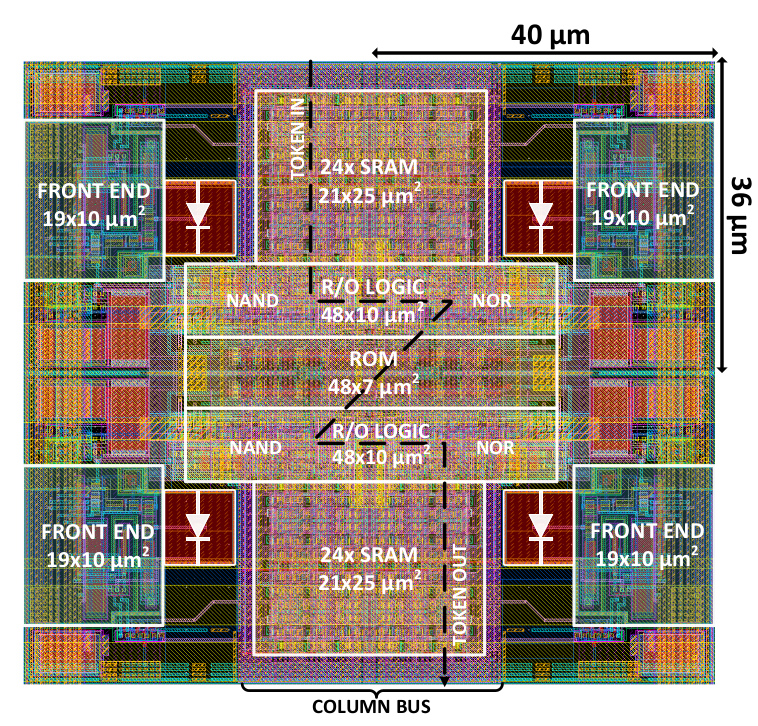
\includegraphics[width=.98\linewidth]{figures/Monopix1/Monopix1_2x2pixelsgroup.png}
    \caption{Layout of a core containing 4 pixels. The analog FE and the digital part are separated in order to reduce cross-talk be}
    \label{fig:pixels_core}
    \end{subfigure}
    \begin{subfigure}{.5\textwidth}
    \centering
    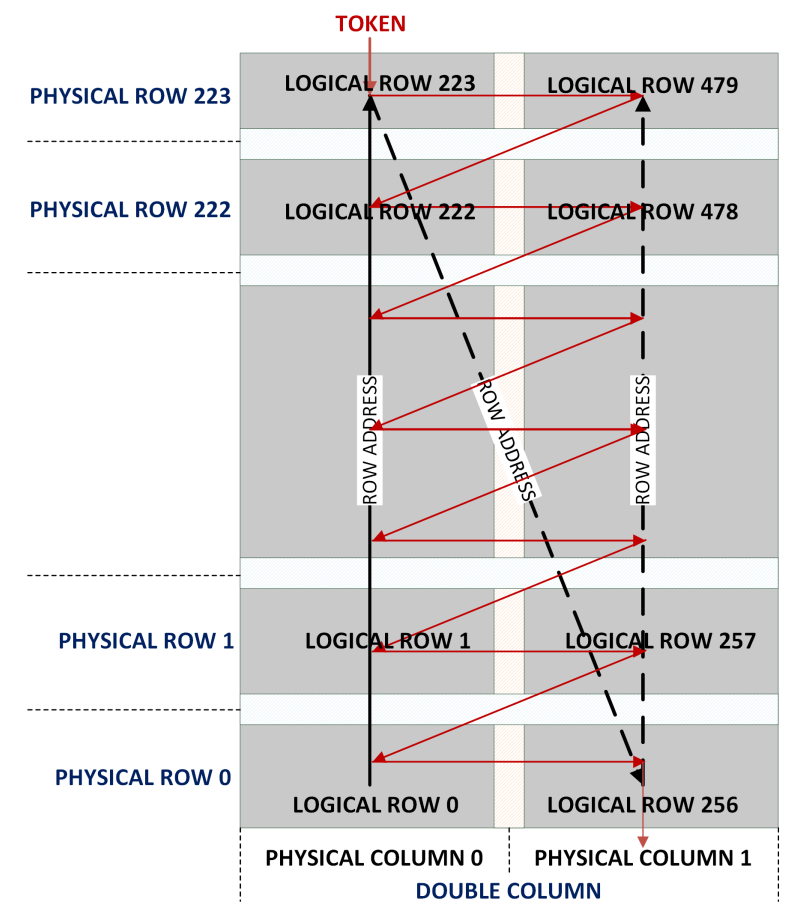
\includegraphics[width=.88\linewidth]{figures/Monopix1/column_order.png}
    \caption{}
    \label{fig:column_order}
    \end{subfigure}
\end{figure}

\begin{table}
    \begin{center}
    \begin{tabular}{| c |c |}
    \hline
    Parameter & Value\\
    \hline
    \hline
    Matrix size &  1$\times$2\si{cm\squared}\\
    Pixel size & 36 $\times$ 40 \si{\um\squared}\\
    Depth & \SI{25}{\um}\\
    Electrode size & \SI{2}{\um}\\
    BCID & \SI{40}{MHz} \\
    ToT-bit & 6 \\
    Power consumption & $\sim$ 120 \si{mW/cm\squared}\\    
    \hline
    \end{tabular}
    \caption{}
    \label{tab:LF-TJ-Monopix}
    \end{center}
\end{table}


\section{The sensor}
    As already anticipated, TJ-Monopix1 has a p-type epitaxial layer and a n doped small collection electrode (\SI{2}{\um} in diameter); to avoid the n-wells housing the PMOS transistors competing for the charge collection, a deep p-well substrate, common to all the pixel FE area, is used.
    TJ-Monopix1 adopts the modification described in section \ref{chap:a_modified_sensor} that allows to achieve a planar depletion region near the electrode applying a relatively small reverse bias voltage.
    This modification improves the efficiency of the detector, especially after irradiation, however a simulation of the electric field in the sensor, made with the software TCAD (Technology Computer Aided Design), shows that a nonuniform field is still produced in the lateral regions of the pixel compromising the efficiency at the corner.
    Two variations to the process have been proposed in order to further enhance the transversal component of electric field at the pixel borders: on a sample of chip, which includes the one in Pisa, a portion of low dose implant has been removed, creating a step discontinuity in the deep p-well corner (fig. \ref{fig:Monopix1_section_scheme}); the second solution proposed\cite{MOUSTAKAS THESYS, PAG 58} consists in adding an extra deep p-well near the pixel edge.
    A side effect of the alteration in the low dose implant is that the separation between the deep p-well and the p-substrate becomes weak to the point that they cannot be biased separately to prevent the punchthrough. 

    \begin{figure}[h!]
        \centering
        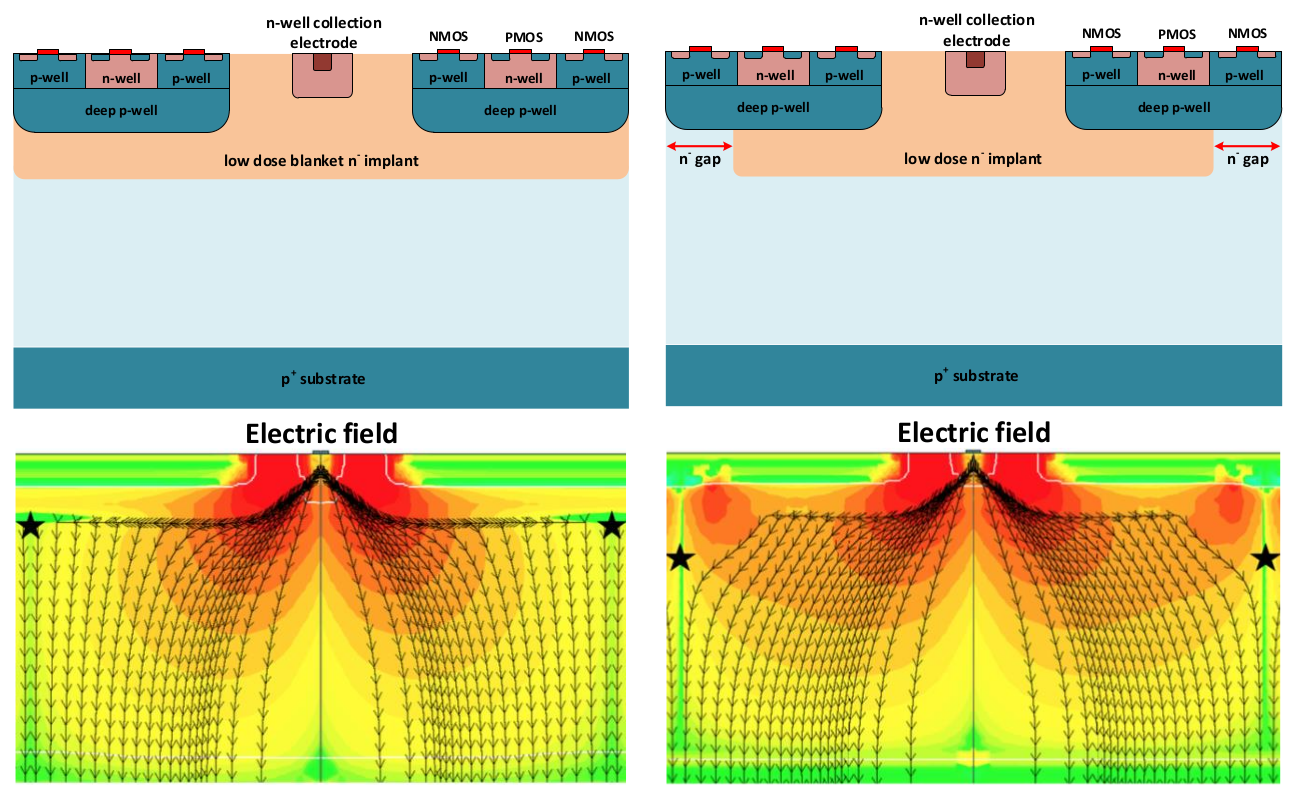
\includegraphics[width=.9\linewidth]{figures/Monopix1/Monopix1_section_scheme.png}
        \caption{(a) The cross-section of a monolithic pixel in the TJ-Monopix with modified process; additionally in (b) a gap in the low dose implant is created to improve the collection of charge due to a bigger lateral component of the electric field. this point in figure  is indicated by a star . transversal component of the electric field drops at the pixel corner}
        \label{fig:Monopix1_section_scheme}
    \end{figure}

    Moreover, to investigate the charge collection properties, pixels within the matrix are split between bottom top half and bottom half and feature a variation in the coverage of the deep p-well: the electronics area can be fully covered or not. In particular the pixels belonging to rows from 0 to 111 are fully covered (FDPW) and pixels belonging to rows from 112 to 223 have a reduced p-well (RDPW), resulting in a enhancement of the lateral component of the electric field.

\section{Front end}
    The matrix is split in four sections, each one corresponding to a different flavor of the FE. The four variation have been implemented in order to test the data-bus readout circuits and the input reset modes.
    \begin{figure}[h!]
        \centering
        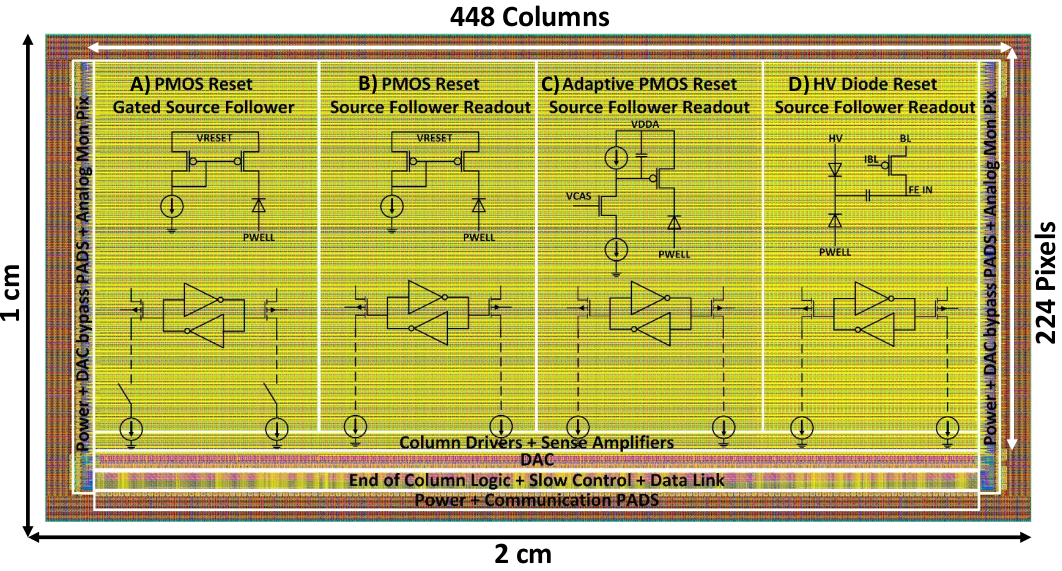
\includegraphics[width=.8\linewidth]{figures/Monopix1/Monopix1_flavors.png}
        \caption{}
        \label{fig:Monopix1_flavors}
    \end{figure}

    All the flavors implement a source-follower double-column bus readout: the standard variation is the flavor B, that features a PMOS input reset (refered as "PMOS reset"). Flavor A is identical to flavor B except for the realization of the source follower (it is a gated one) that aim to reduce the power consumption.\red{cosa significa?} C instead implements a novel leakage compensation circuit.
    Moreover the collection electrode in flavors A, B, C is DC-coupled to the front-end input, while in D is AC-coupled, providing to applu a high bias voltage; for this reason flavor D il called "HV flavor".

    \red{Principio generale: R resistenza di reset deve essere abbastanza grande in modo da far si che il ritorno allo zero è abbastanza lento (non devi "interferire" con la tot slope e non deve essere più corto del tempo del preamplificatore, sennò hai perdita di segnale).
    Baseline reset: all'input solitamente hai un PMOSS o un diodo;  
    R reset}

    \subsection{ALPIDE-like}
        ALPIDE chips, developed by the ALICE collaboration, implemented a standard FE to the point that many CMOS MAPS detectors used a similar FE and are called "ALIPDE-like". 
        Concidering that both TJ-Monopix1 and ARCADIA-MD1 have an ALPIDE-like FE, I am going to explain the broad principles of the early FE stage. 
        \begin{figure}[h!]
            \begin{subfigure}{.5\textwidth}
            \centering
            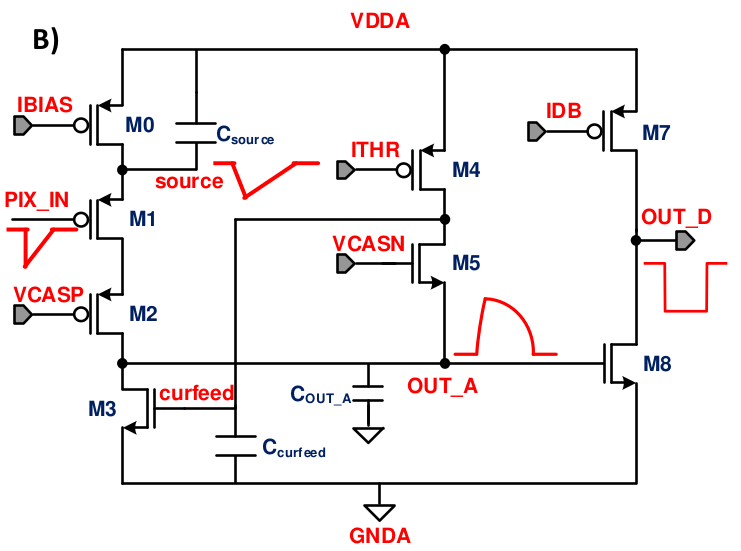
\includegraphics[width=.98\linewidth]{figures/Monopix1/ALPIDE_FE.png}
            \caption{ALPIDE-like}
            \label{fig:ALPIDE-like}
            \end{subfigure}
            \begin{subfigure}{.5\textwidth}
            \centering
            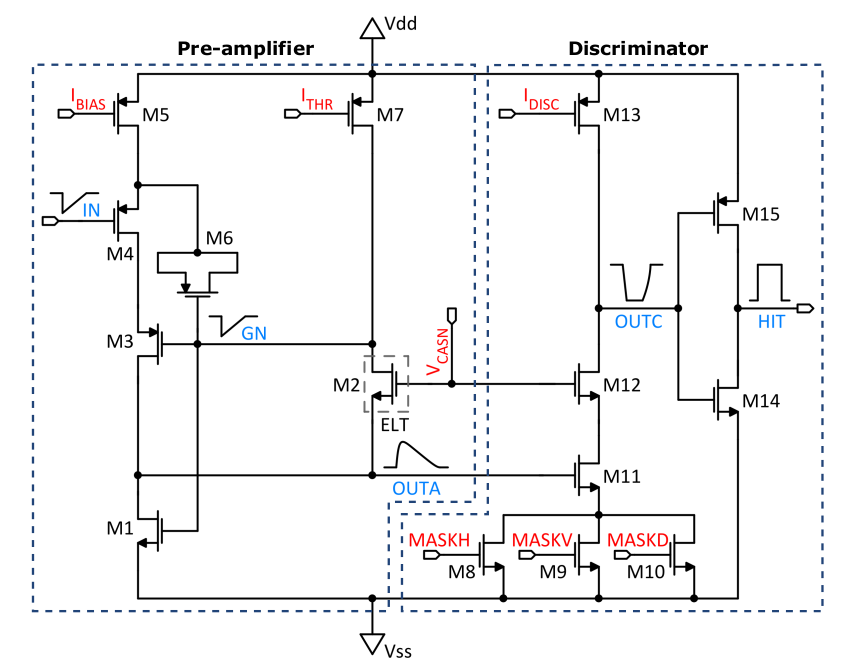
\includegraphics[width=.98\linewidth]{figures/Monopix1/Monopix1_FE_circuit.png}
            \caption{}
            \label{fig:Monopix1_FE_circuit}
            \end{subfigure}
        \end{figure}
        The general idea is of the amplification to transfer the charge from a bigger capacity\cite{ALPIDE-FE}, $C_{source}$, to a smaller one, $C_{out}$: the input transistor M1 with current source IBIAS acts as a source follower and this forces the source of M1 to be equal to the gate input  $\Delta V_{PIX\_IN} = Q_{IN}/C_{IN}$.
        \begin{equation}
            Q_{source} = C_{source} \Delta V_{PIX\_IN}
        \end{equation}
        The current in M2 and the charge accumulates on $C_{out}$ is fixed by the one on $C_{source}$:
        \begin{equation}
            \Delta V_{OUT\_A} = \frac{Q_{source}}{C_{OUT\_A}} = \frac{C_{source}\Delta V_{PIX\_IN}}{C_{OUT\_A}}  = \frac{C_{Source}}{C_{OUT\_A}}\frac{Q_{IN}}{C_{IN}}
        \end{equation}
        A second branch (M4, M5) is used to generate a low frequency feedback, where VCASN and ITHR set the baseline value of the signal on $C_{OUT\_A}$ and the velocity to goes down to the baseline.\\
        \red{IL RUOLO DI CURVFEED NON L'HO CAPITO.}\\
        Finally IDB defines the charge threshold with which the signal $OUT\_A$ must be compared: depending on if the signal is higher than the threshold or not, the $OUT\_D$ is high or low respectively.

        The actual circuit implemented in TJ-Monopix1 is shown in figure \ref{fig:Monopix1_FE_circuit}: the principal difference lays in the addition of disableing pixels' readout. This possibility is uttermost important in order to reduce the hit rate and to avoid saturating the bandwidth due to the noisy pixels, which typically are those with manufacturing defects.
        In the circuit transistors M8, M9 and M10 have the function of disabling registers with coordinates MASKH, MASKV and MASKD (respectivelly vertical, orizontal and diagonal) from readout: if all three transistors-signals are low, the pixel's discriminator is disabled. 
        Compared with a configurable masking register which would allow disableing pixels individually, to use a triple redundancy reduces the sensistivity to SEU but also gives amount of intentionally masked ("ghost") pixels.
        This approach is suitable only for extremely small number N of pixel has to be masked: if two coordinate projection scheme had been implemented, the number of ghost pixels would have scale with $N^2$, if instead three coordinates are used, the N's exponential is lower than 2 (fig. \ref{fig:masking_scheme})
        \begin{figure}[h!]
            \centering
            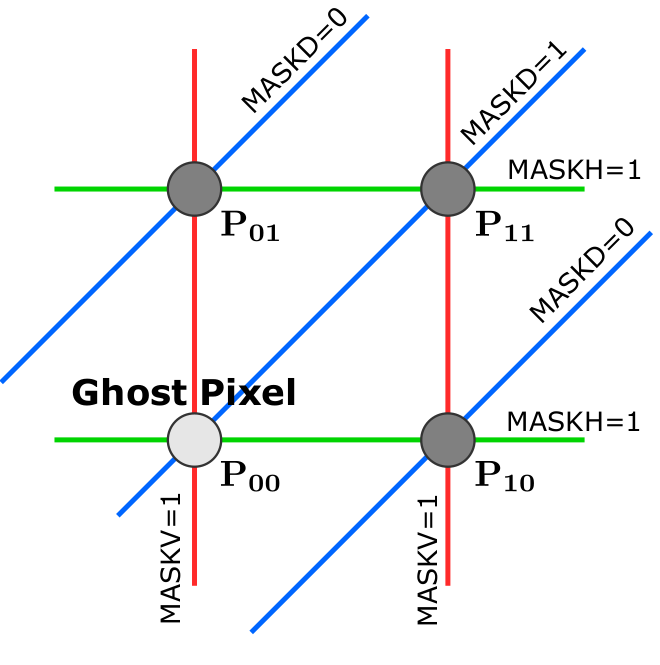
\includegraphics[width=.3\linewidth]{figures/Monopix1/masking_scheme.png}
            \caption{}
            \label{fig:masking_scheme}
        \end{figure}

        \begin{table}
            \begin{center}
            \begin{tabular}{|c | c | c |}
            \hline
            Parameter & Meaning & \\
            \hline
            \hline
            IBIAS & mainly controls the rise time & \red{yes? check}\\
            IDB & sets the discriminator threshold & yes\\
            ITHR & sets the velocity of the return to the baseline & yes \\
            ICASN & sets the baseline of the signal & yes\\
            VRESET & sets the gain of the preamplifier & yes\\
            IRESET & sets the gain of the preamplifier & no\\
            \hline
            \end{tabular}
            \caption{FE parameters which must be setted through the DAQ. "Function" means that higher parameter implies higher value}
            \label{tab:FE-parameters}
            \end{center}
        \end{table}
    


\section{Readout logic}
    TJ-Monopix1 has a triggerless, fast and with ToT capability R/O which is based on a column-drain architecture.      
    On the pixel are located two Random Access Memory (RAM) cells to store the 6-bit LE and 6-bit TE of the pulse, and a Read-Only Memory (ROM) containing the 9-bit pixel address. Excluded these memories, TJ-Monopix1 hasn't any other buffer: if a hit arrives while the pixel is already storing a previous one, the new data get lost.  
    After being read, the data packet is sent to the EoC periphery of the matrix, where a serializer transfers it off-chip to an FPGA (\ref{fig:R/O-system}). There a FIFO is used to temporarily stored the data, which is transmitted to a computer through an ethernet cable in a later time.  
    \begin{figure}
        \begin{subfigure}{\textwidth}
        \centering
        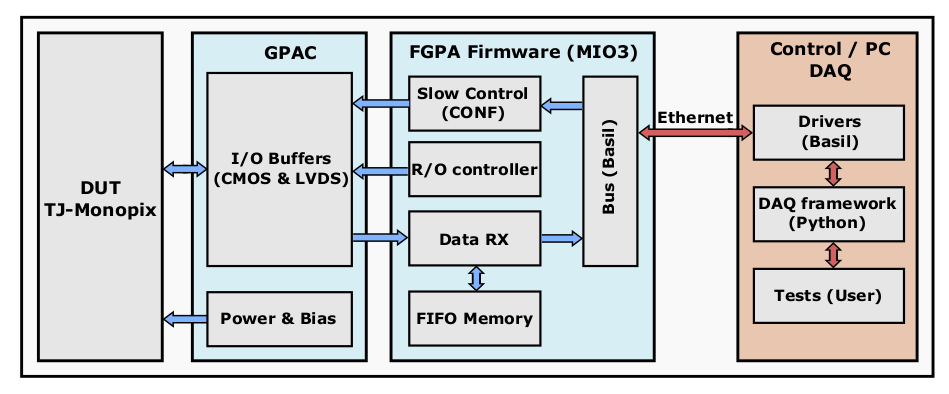
\includegraphics[clip,width=0.8\linewidth]{figures/Monopix1/schematic_boards.png}
        \end{subfigure}
        \bigskip
        \begin{subfigure}{\textwidth}
        \centering    
        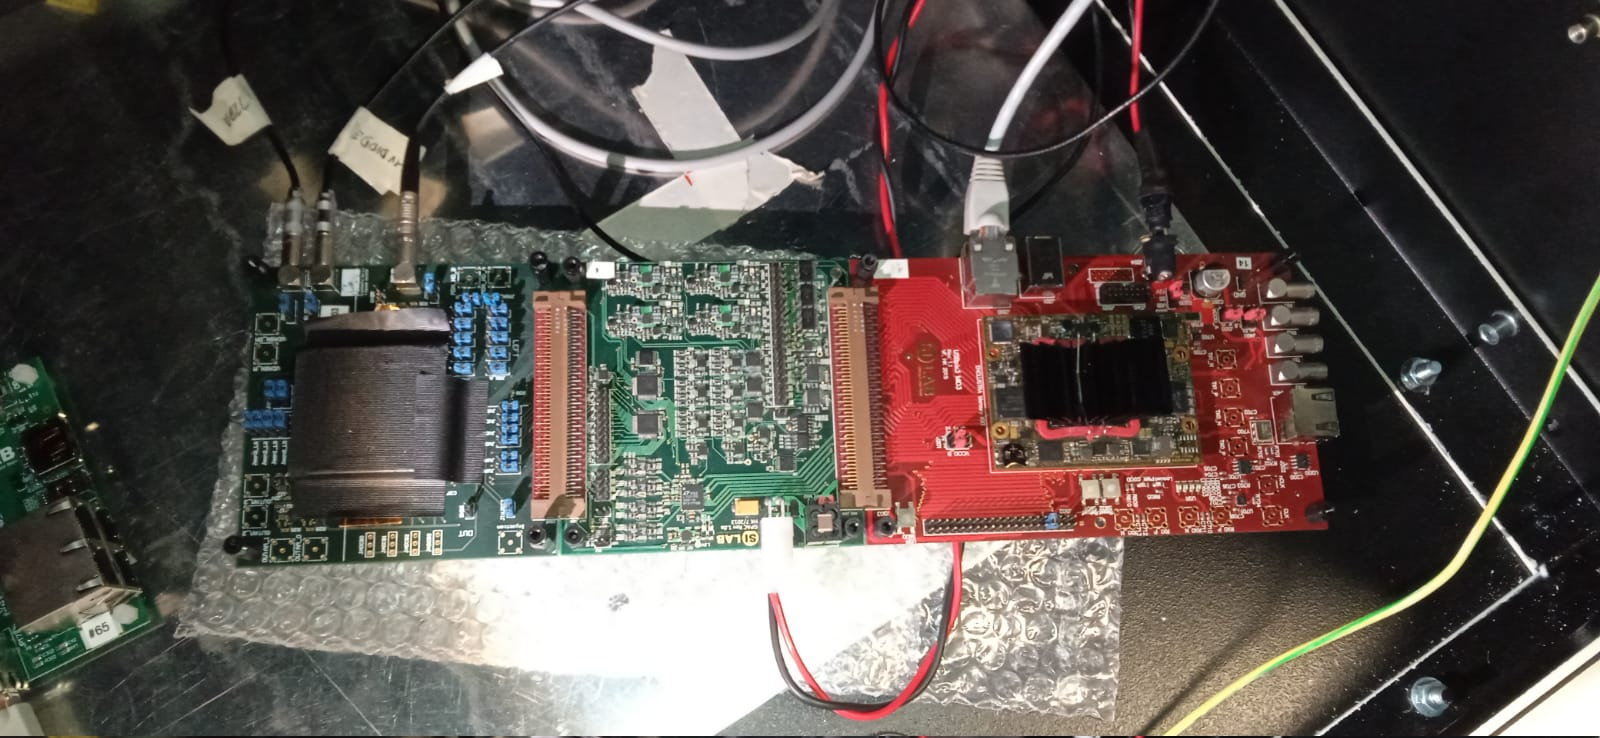
\includegraphics[clip,width=0.8\linewidth]{figures/Monopix1/monopix1_front.jpeg}
        \end{subfigure}
        \caption{Main caption}
        \label{fig:R/O-system}
    \end{figure}


    The access to the pixels' memory and the transmission of the data to the EoC, following a priority chain, is managed by control signals and is based on a Finite State Machine (FSM) composed by four state: no-operation (NOP), freeze (FRZ), read (RD) and data transfer (DTA). The readout sequence (\ref{fig:readout_schematics}) starts with the TE of a pulse: the pixel immediately tries to grab the column-bus turning up a hit flag signal called \textit{token}.   
    The token is used to control the priority chain and propagates across the column indicating what pixel that must be read. To start the readout and avoid that the arrival of new hits disrupt the priority logic, a \textit{freeze} signal is activated, and then a \textit{read} signal controls the readout and the access to memory.
    During the freeze, the state of the token for all pixels on the matrix remains settled: this does not forbid new hits on other pixels from being recorded, but forbids pixels hit from turning on the token until the freeze is ended. 
    The freeze stays on until the token covers the whole priority chain and gets the EoC: during that time new token cannot be turned on, and all hits arrived during a freeze will turn on their token at the end of the previous freeze.  
    Since the start of the token is used to assign a timestamp to the hit, the token time has a direct impact on the time resolution measurement; this could be a problem coping with high hits rate. 
    \begin{figure}[h!]
        \centering
        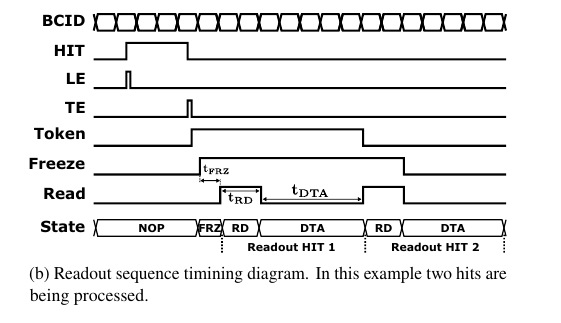
\includegraphics[width=.5\linewidth]{figures/Monopix1/readout_timing.png}
        \caption{Readout timing diagram: in this example two hits are being processed}
        \label{fig:readout_timing}
    \end{figure}

    The analog FE circuit and the pixel control logic are connected by an edge detector which is used to determine the LE and the TE of the hit pulse(fig. \ref{fig:pixel_logic}): when the TE is stored in the first latch the edge detector is disabled and, if the \textcolor{red}{FREEZE} signal is not set yet, the readout starts. 
    At this point the HIT flag is set in a second latch and a token signal is produced and depending on the value of \textcolor{Cerulean}{Token in} the pixel can be read or must wait until the \textcolor{Cerulean}{Token in} is off. In figure an OR is used to manage the token propagation, but since a native OR logic port cannot be implemented with CMOS logic, a sum of a NOR and of an inverter is actually used; this construct significantly increases the propagation delay (the timing dispersion along a column of 0.1-0.2 ns) of the token and to speed up the circuit optimized solution are often implemented.  
    When the pixel become the next to be read in the queue, and at the rising edge of the \textcolor{red}{READ} signal, the state of the pixel is stored in a D-latch and the pixel is allowed to use the data bus; the TE and the HIT flag latches are reset and a \textcolor{Cerulean}{READINT} signal that enable access of the RAM and ROM cells is produced.\\
    \begin{figure}[h!]
        \centering
        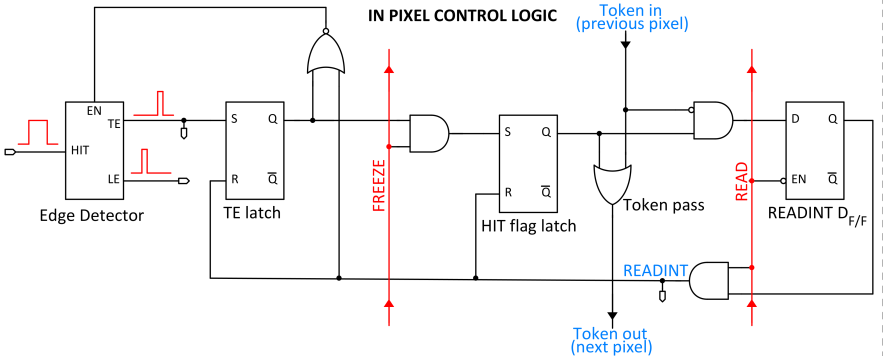
\includegraphics[width=.9\linewidth]{figures/Monopix1/Monopix1_readout_schematics.png}
        \caption{}
        \label{fig:pixel_logic}
    \end{figure}
    
    The final data must provide all the hits' information: the pixel address, the ToT and the timestamp. All those parts are assigned and appended at different time during the R/O chain:  
    \begin{itemize}
        \item\textbf{Pixel address:} while the double column address (6-bit) is appended by the EoC circuit, the row address (8-bits for each flavor) and the physical column in the doublet (1-bit) are assigned by the in-pixel logic      
        \item \textbf{ToT:} is obtained offline from the difference of 6-bits TE and 6-bits LE, stored by the edge detector in-pixel; since a 40 MHz BCID is distributed across the matrix, the ToT value is range 0-64 clock cycle which corresponds to 0-1.6 \si{\us}  
        \item \textbf{Timestamp:} The timestamp of the hit correspond to the time when the pixel set up the token; it is assigned by the FPGA, that uses the LE, TE and a 640 MHz clock to derive it. For all those hits which arrived while the matrix is frozen, the timestamp is no more correlated with the time of arrival of the particle         
    \end{itemize}
    When the bits are joined up together the complete hit data packet is 27-bit. 


 
        \begin{figure}[h!]
            \centering
            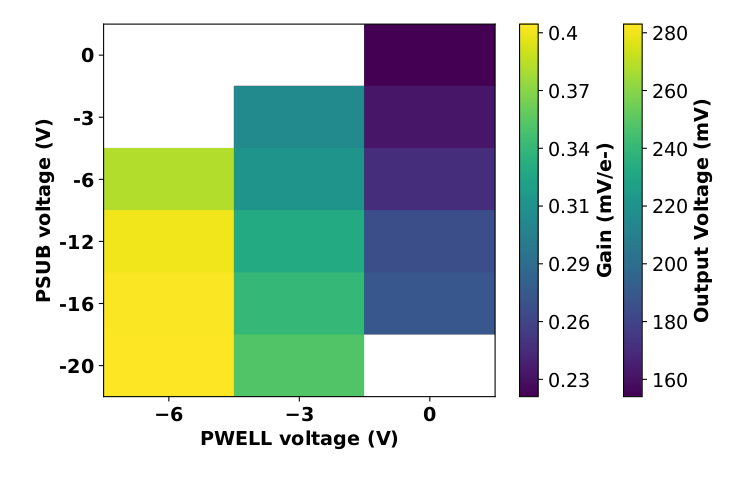
\includegraphics[width=.40\linewidth]{figures/Monopix1/gain_vs_bias.png}
            \caption{2D map of the output voltage amplitude and gain with respect to the p-well and p-substrate in the case of the PMOS reset front-end }
            \label{fig:gain_vs_bias}
        \end{figure}      
        \red{Measurement of the magnitude of the collected charge
        has also been generally available for pixel detectors, and has
        been used to improve the 3D space point precision through
        interpolation as well as for particle identification through spe-
        cific ionization measurement.}
    
    

